\section{Hardware Demonstrations}\label{sec:hardware}
\begin{figure*}[t]
    \centering
    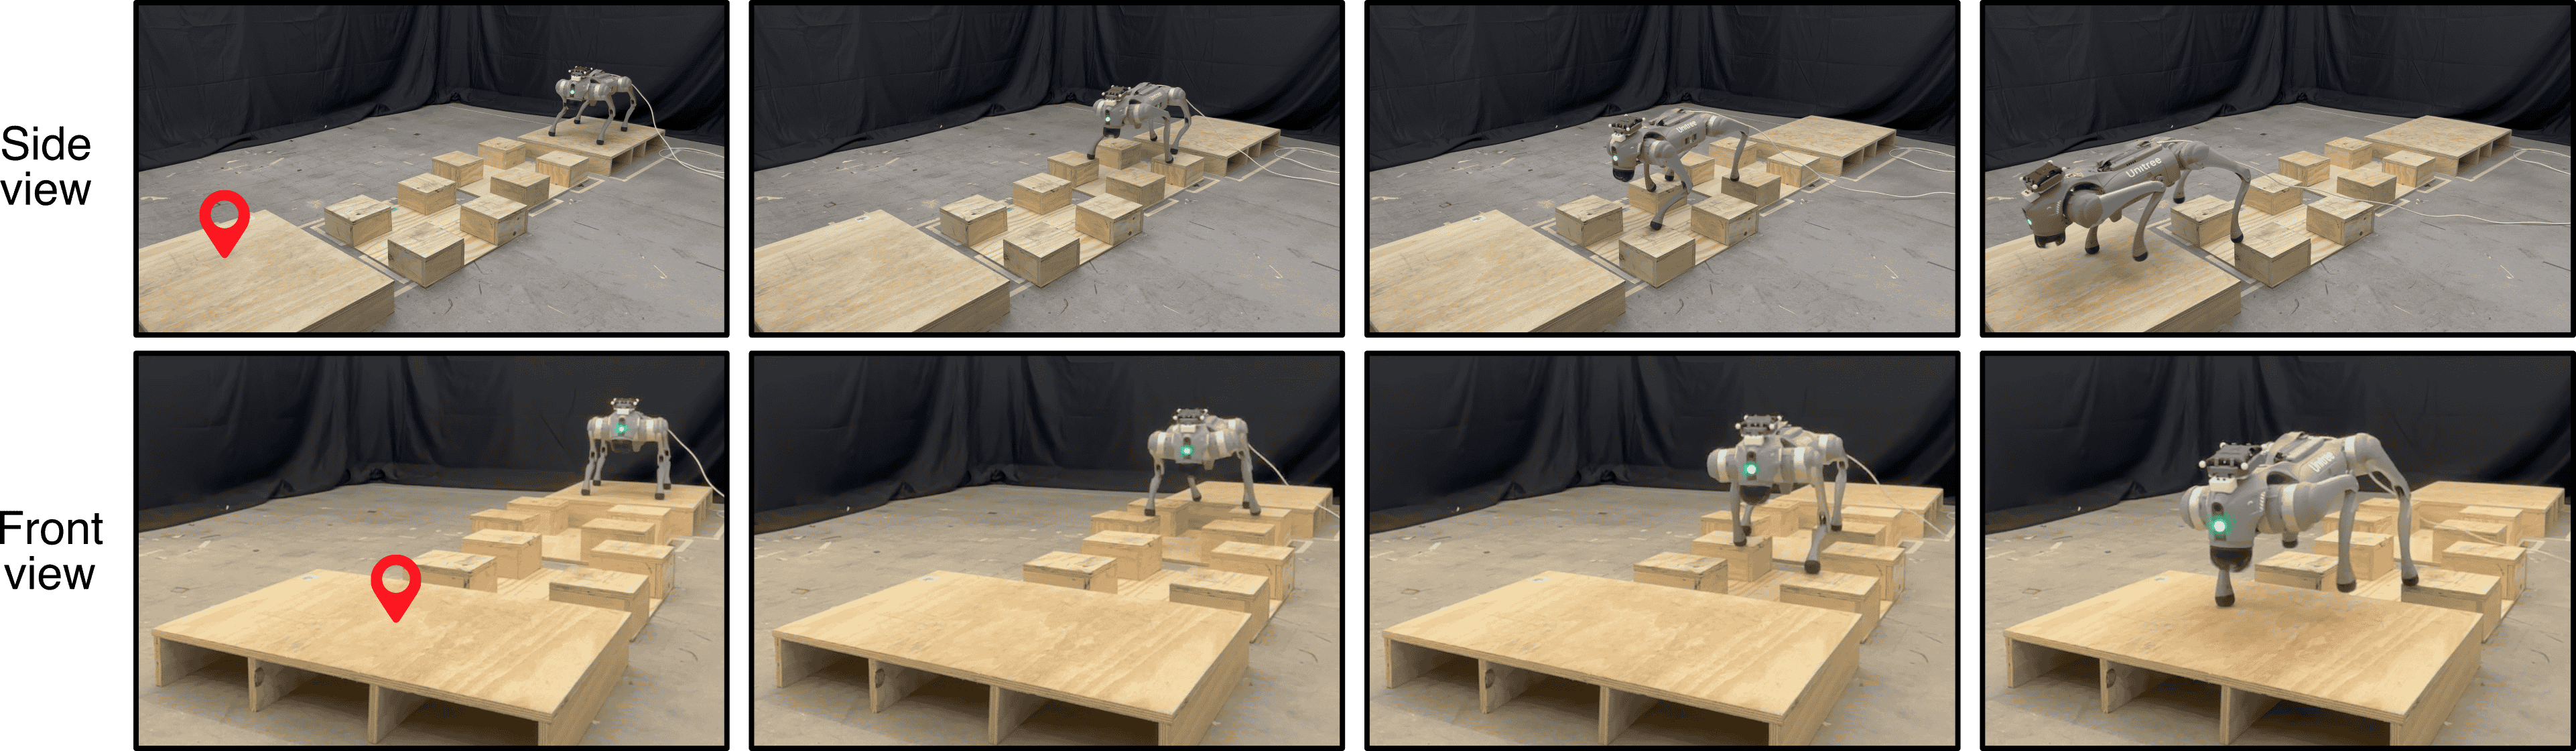
\includegraphics[width=\linewidth]{unstructured_hardware_withoutgap_compressed.png}
    \caption{Hardware experiment on the first unstructured-terrain scenario: sparse stepping stones ($0.18$--$0.23$\,m apart) interleaved with flat regions. Side and front views highlight the lateral misalignment of the stones; the online MICP produces a sideways trajectory and a $3$\,s trotting gait is used throughout.}
    \label{fig:hardware_withoutgap}
\end{figure*}
We demonstrate that our entire framework can be successfully deployed on hardware, highlighting two key aspects. First, we showcase the framework’s capability to generate adaptive locomotion gaits across diverse terrain types, particularly focusing on agile leaping motions. Second, we illustrate the framework’s assured safety through obstacle avoidance and selection of dynamically feasible gaits, benchmarked against a heuristic-based planner.
\subsection{Hardware Experiment Setup}
For hardware experiments, we set up similar real-world scenarios for both unstructured and rebar terrains. For the unstructured terrain scenario, we construct wooden blocks to form stepping stones, gaps, and flat regions, with each stepping stone elevated approximately $0.12$ m above the ground. For the rebar scenario, we assemble a realistic rebar mat using fourteen $1/2$-inch $\times$ $4$-foot rebars and six $1/2$-inch × $10$-foot rebars.
In the synthesis setup, obstacles are considered a distinct terrain type, consistent with the simulation. Both scenarios assume the maximum potential terrain types—8 for unstructured and 14 for rebar—though the real setups include fewer types. As demonstrated in the simulation, this does not increase complexity, as it only scales linearly with terrain-request pairs due to our high-level manager.
For safety, we set abstraction cell sizes to $0.8$ m for the unstructured terrain and $0.45$ m for the rebar terrain.

\subsection{Unstructured Terrain}
As shown in Fig.~\ref{fig:hardware_withoutgap}, we first create a scenario with sparse stepping stones and flat terrain regions. The stepping stones are spaced between $0.18 - 0.23$ m apart. Both side and front views are provided to highlight the misalignment of stepping stones along the robot walking direction. %\ye{[check if this change makes sense]}\ziyi{[LGTM]} 
The MICP planner successfully generates a reference trajectory involving non-trivial sideways movement, enabling the robot to safely land on the stepping stones. All transitions utilize a $3$ s trotting gait. 

In the second scenario, shown in Fig.~\ref{fig:hardware_withgap}, we further include a gap terrain segment. The gap, approximately 30 cm wide, necessitates the use of a leaping gait. Since the gap terrain was incorporated during offline synthesis, our framework can directly select an optimized $1.5$ s leaping gait generated by gait-free MICP upon encountering this gap terrain. The task-space tracking performance between the measured state and the reference trajectory generated by the online MICP is shown in Fig.~\ref{fig:tracking_performance}. This includes the floating base position and the end-effector (EE) position for the front-left foot. The EE tracking maintains errors within $0.01$ m in the x and y axes, ensuring precise foot placement. Meanwhile, the NMPC effectively adjusts the base position to compensate for model simplifications at the MICP level, enabling successful execution of both trotting and leaping motions.
\begin{figure}
    \centering
    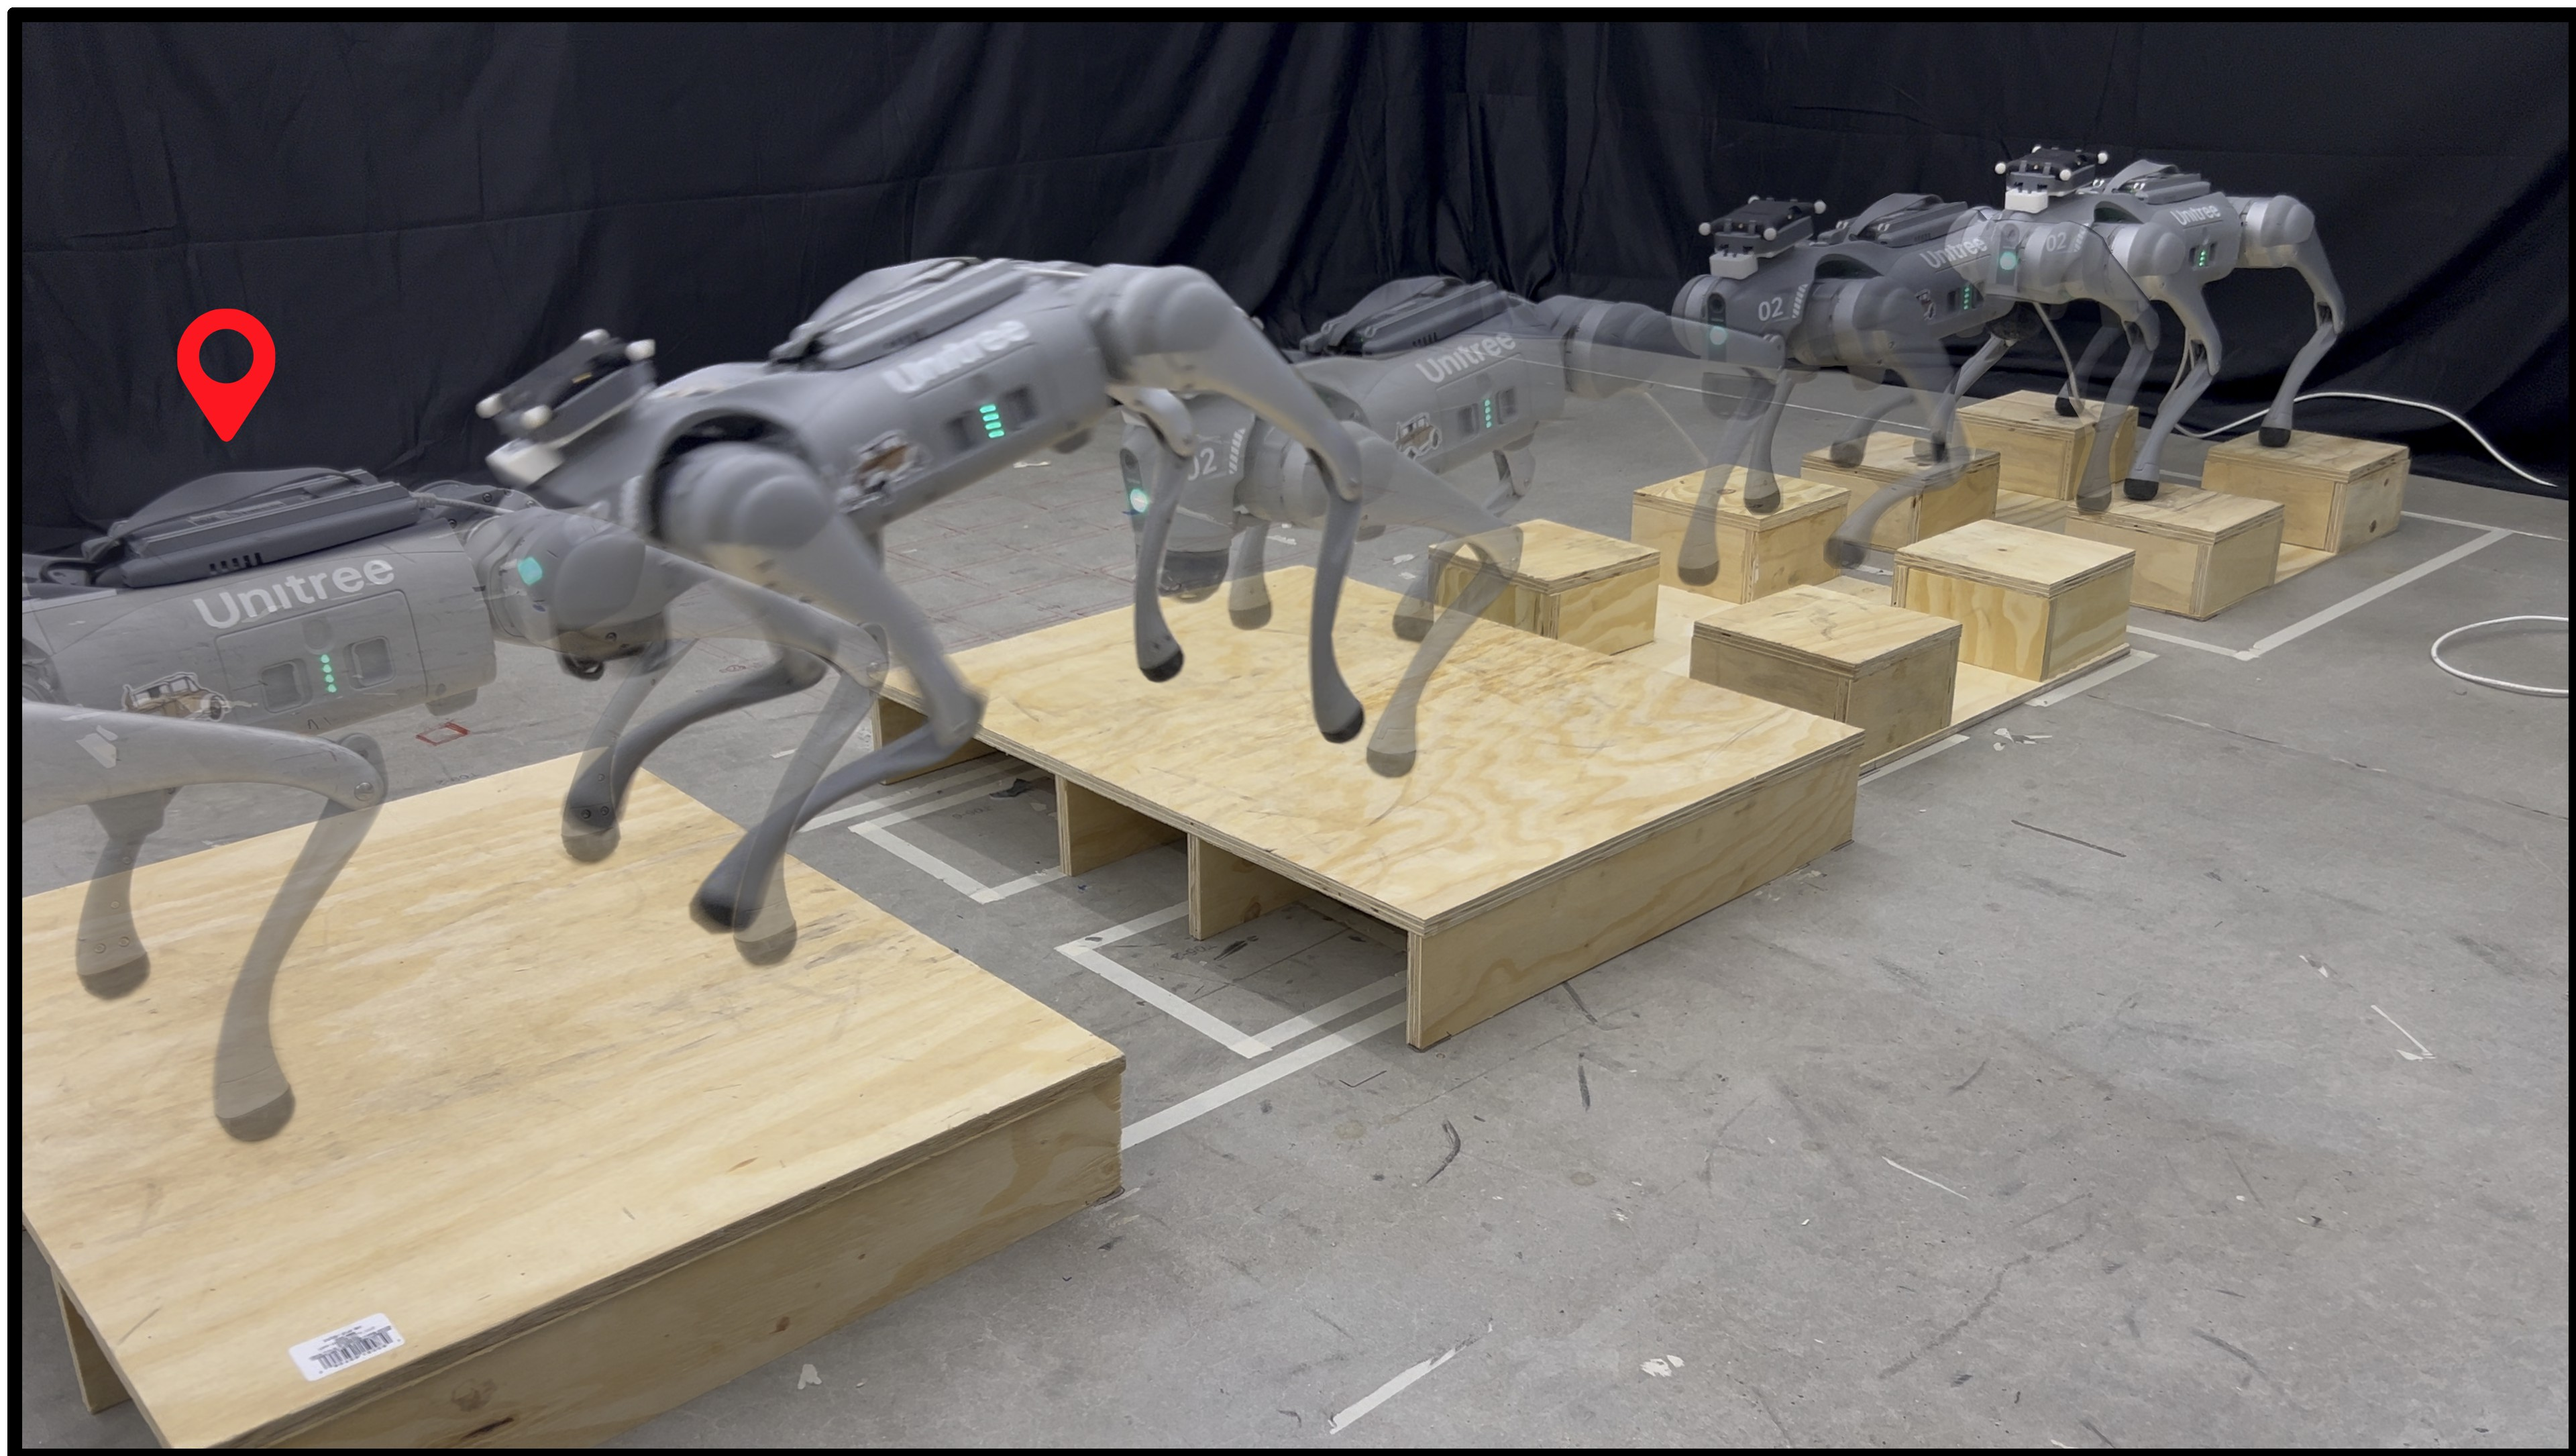
\includegraphics[width=\linewidth]{unstructured_hardware_withgap.jpg}
    \caption{Hardware experiment demonstration for the second unstructured terrain scenario with sparse stepping stones, flat, and gap terrains.}
    \label{fig:hardware_withgap}
\end{figure}
\begin{figure}
    \centering    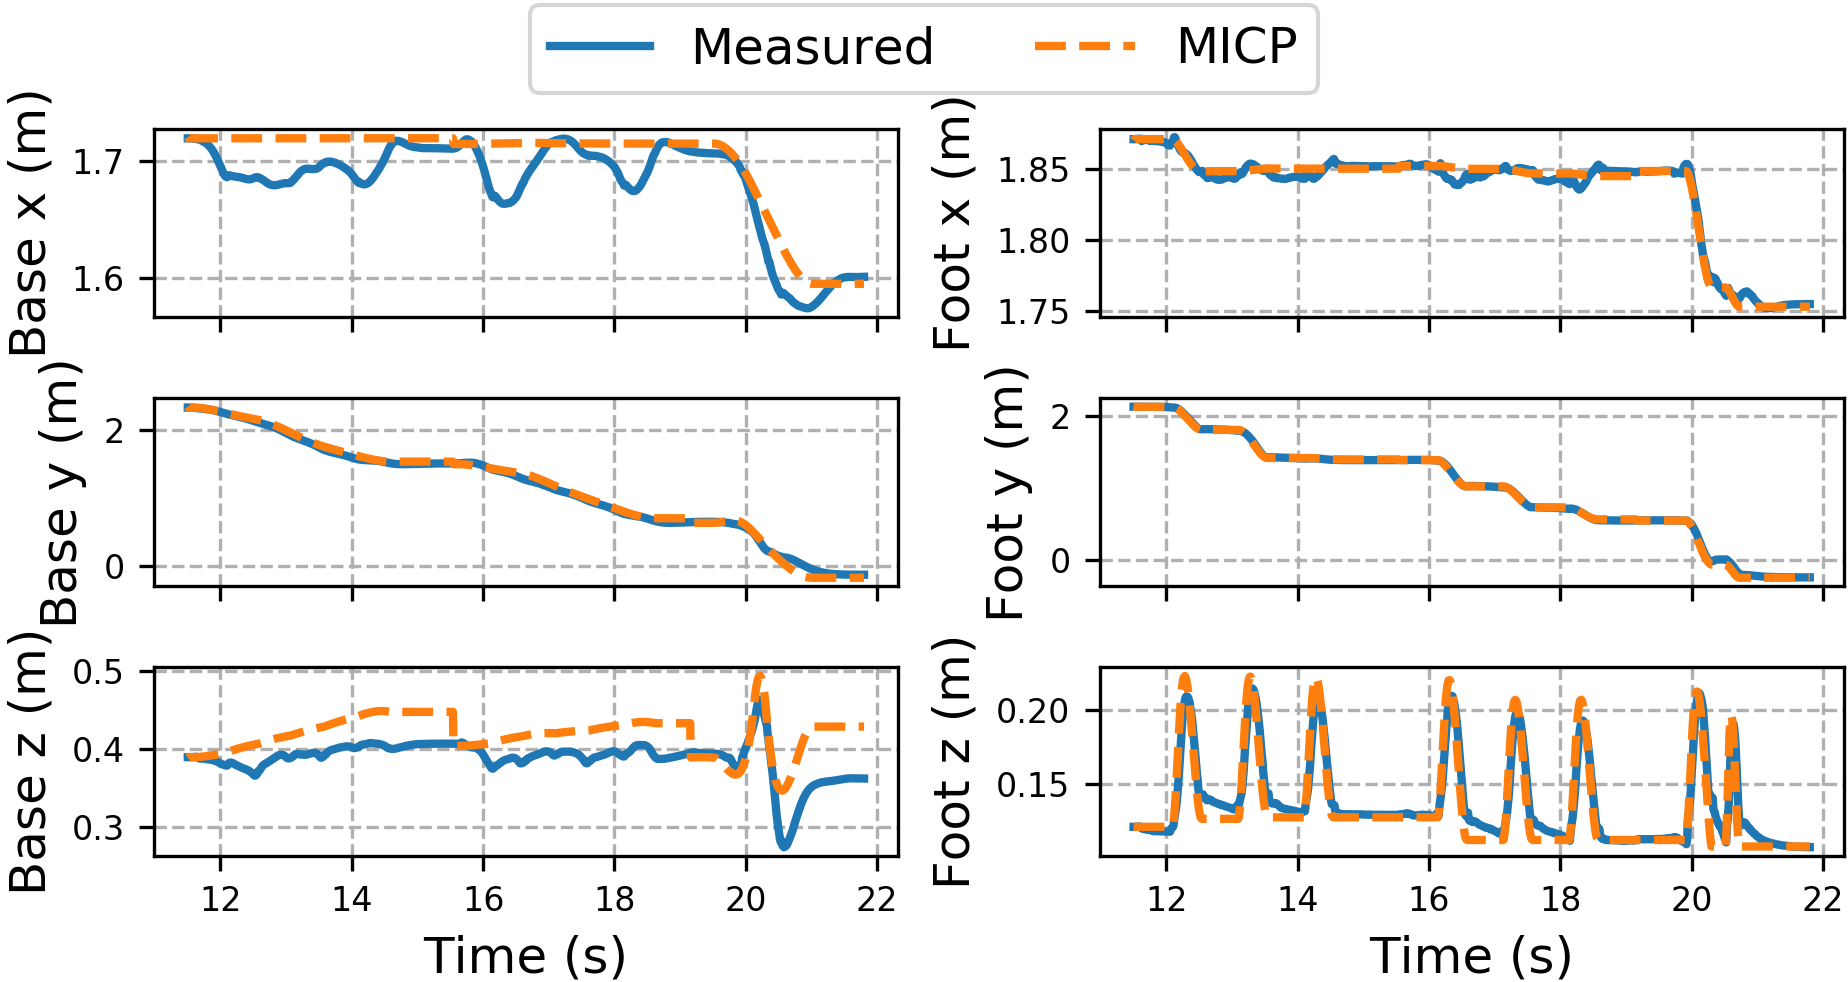
\includegraphics[width=\linewidth]{tracking_performance.png}
    \caption{Tracking performance of the base and front-left foot positions: comparison between measured states and MICP-generated reference trajectories.}
    \label{fig:tracking_performance}
\end{figure}
\subsection{Rebar Terrain}\label{subsec:rebar_terrain}
\begin{figure*}[t]
    \centering
    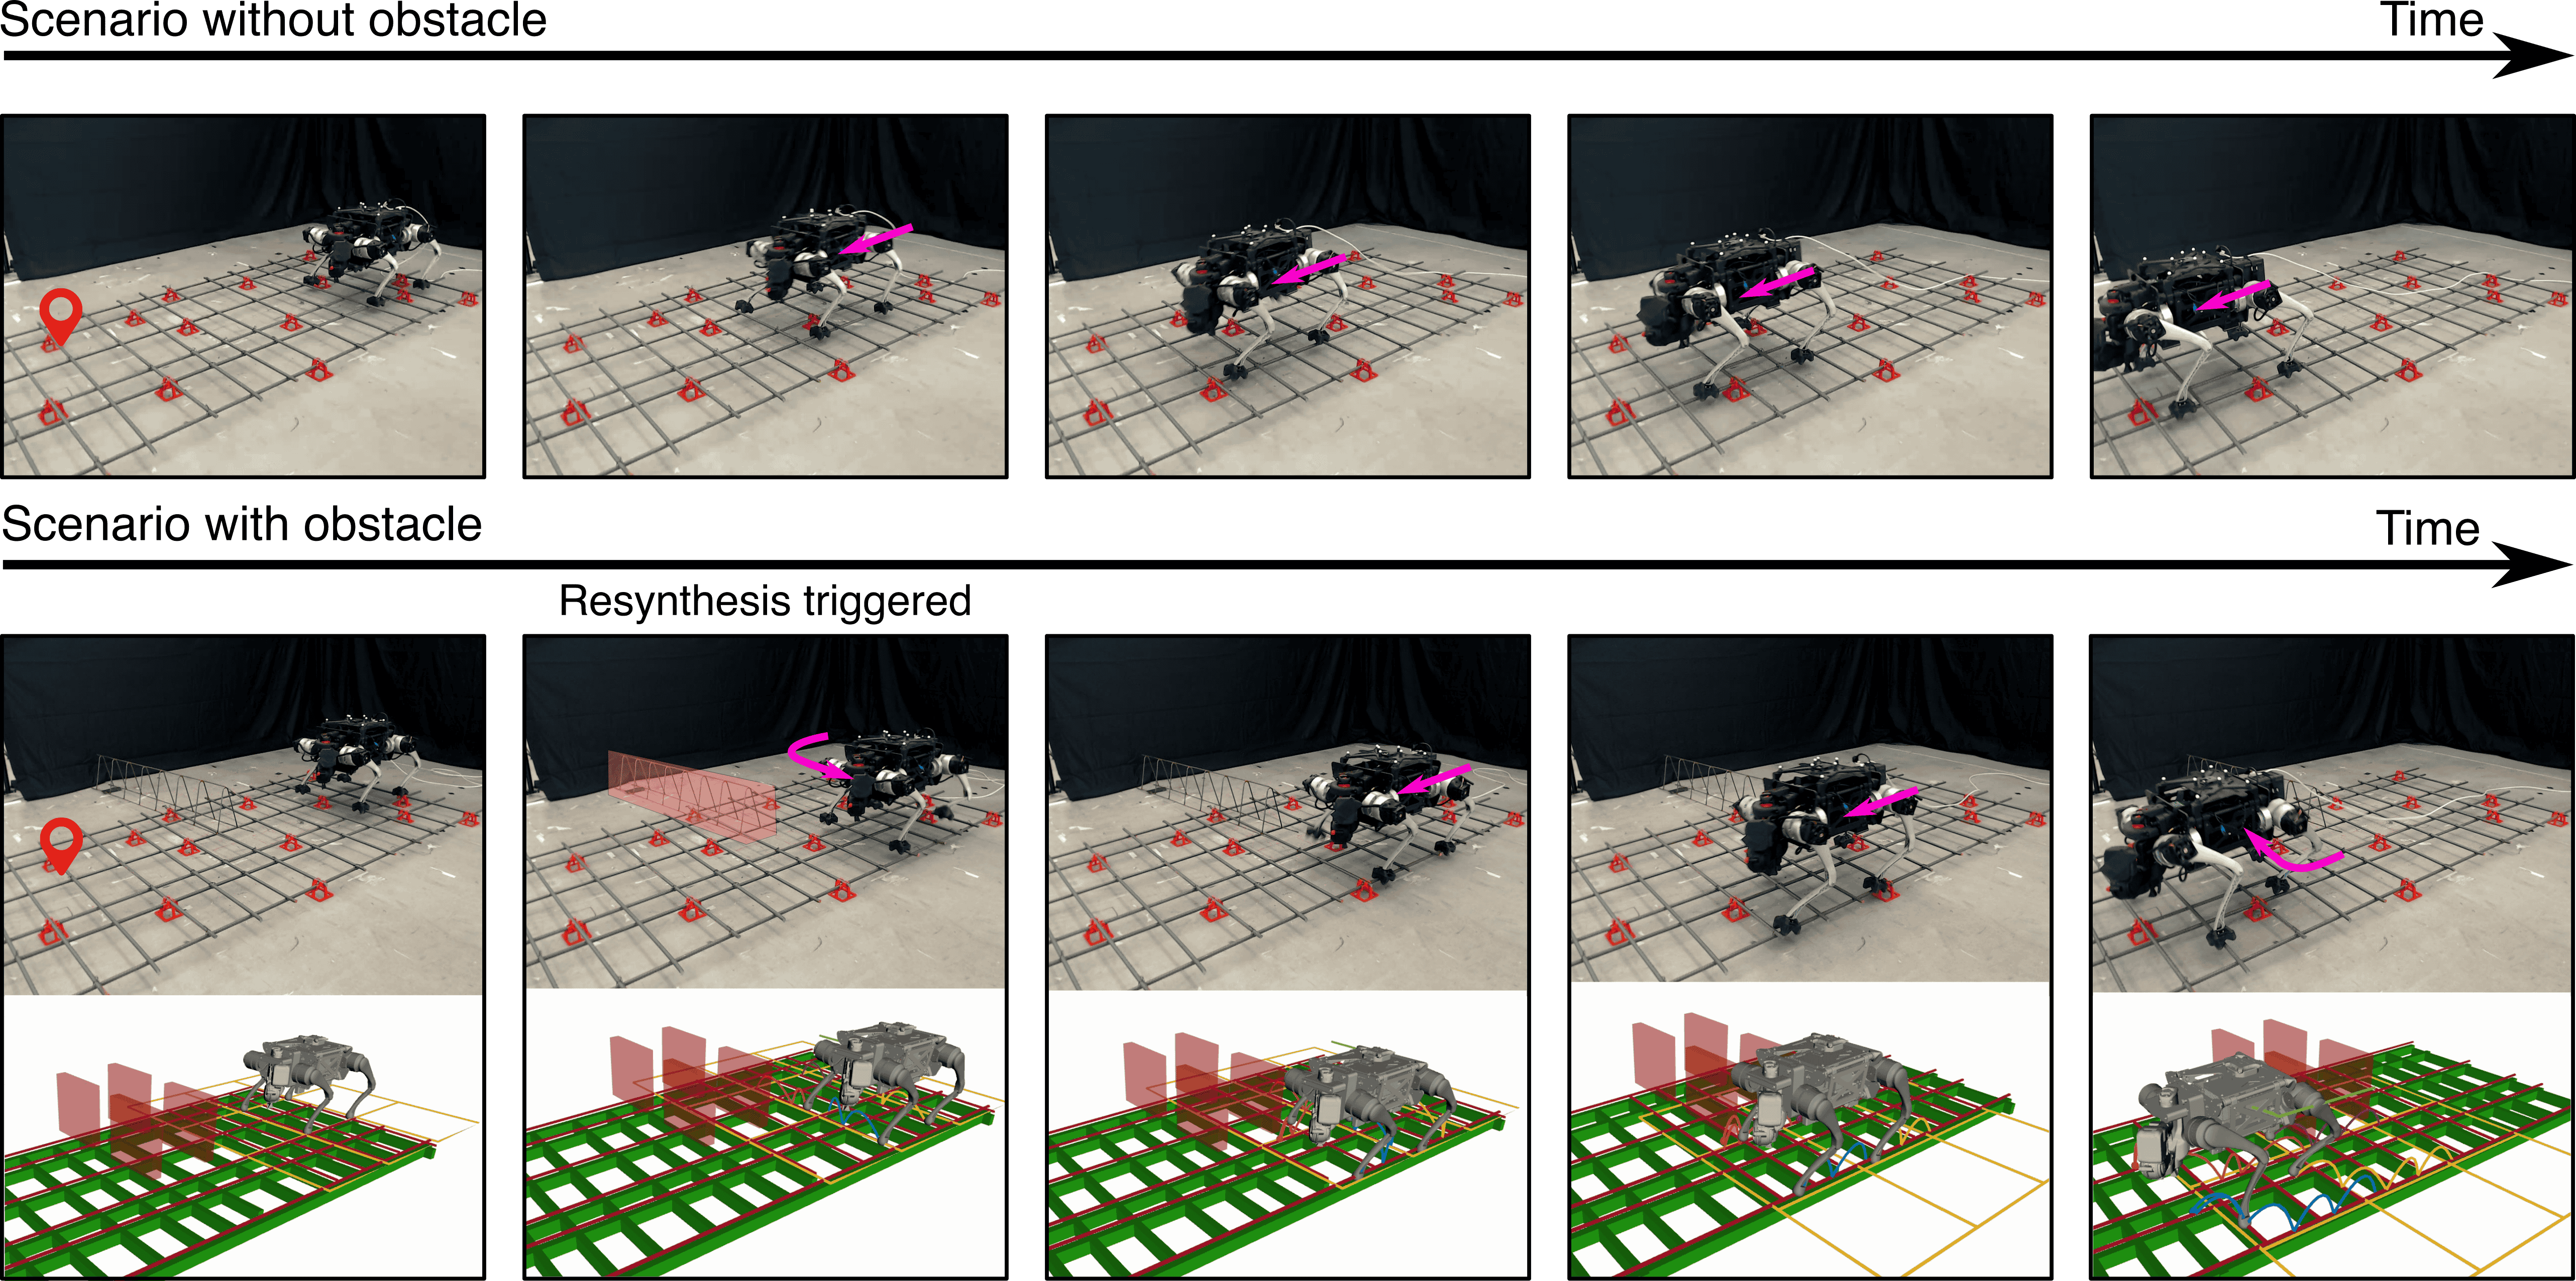
\includegraphics[width=\linewidth]{hardware_rebar_compressed.png}
    \caption{Execution results in rebar terrain without (top row) and with obstacle (bottom row). In the obstacle case, runtime resynthesis is triggered to generate a detour strategy and ensure successful traversal.}
    \label{fig:hardware_rebar}
\end{figure*}
For the rebar terrain scenarios shown in Fig.~\ref{fig:hardware_rebar}, we test two cases: one without any obstacles and one with an obstacle introduced during execution. The rebar spacing varies between $0.1$ m and $0.3$ m. Offline synthesis is conducted without prior knowledge of obstacles. In the first case (top row), the robot Chotu successfully performs the entire maneuver without encountering any runtime failures, consistently moving forward until reaching the goal waypoint.
In the second case (bottom row), an obstacle is added to the environment but only detected during the online execution phase. \revised{In our hardware setup, the obstacle's location is not estimated by an autonomous perception stack but rather provided through motion-capture-aided manual annotation: when the obstacle enters the robot's local field of view, its position is added to the online terrain set and the affected cell is classified as the \textit{obstacle} terrain class at the symbolic level---i.e., obstacle avoidance in this scenario is handled entirely at the symbolic level (Sec.~\ref{sec:preliminaries_abstraction}), not through the MICP-level collision-region variables $\v H_{s,w,j}$ in Eq.~(\ref{eq:collision_avoidance}). This setup is explicit about what is and is not validated---the planning and runtime-repair pipeline is exercised end-to-end, while the terrain-segmentation problem itself is not.} Upon encountering a new terrain/request pair caused by the obstacle, the planner promptly triggers a runtime resynthesis. Leveraging previously generated skills, it computes a new strategy within $0.05$ s to detour around the obstacle and continue toward the goal. All transitions in both scenarios use a $2.25$ s static walking gait, where only one foot is lifted at a time to ensure safety. \revised{We note that the gait timings adopted on hardware---$3$\,s trotting, $1.5$\,s leaping, $2.25$\,s static walking---are conservative compared to the most agile motions reported in the legged-locomotion literature; however, this locomotion gait setup still verifies the framework's gait-switching, online MICP, and runtime-repair mechanisms, which is the validation target of this article. Aggressive, high-speed gaits would require revisiting the convex-dynamics simplification (Eq.~(\ref{eq:dynamics})) discussed in Sec.~\ref{sec:online_execution}.}


\subsection{Benchmark: Heuristics-Based Planner}
\begin{figure*}
    \centering
    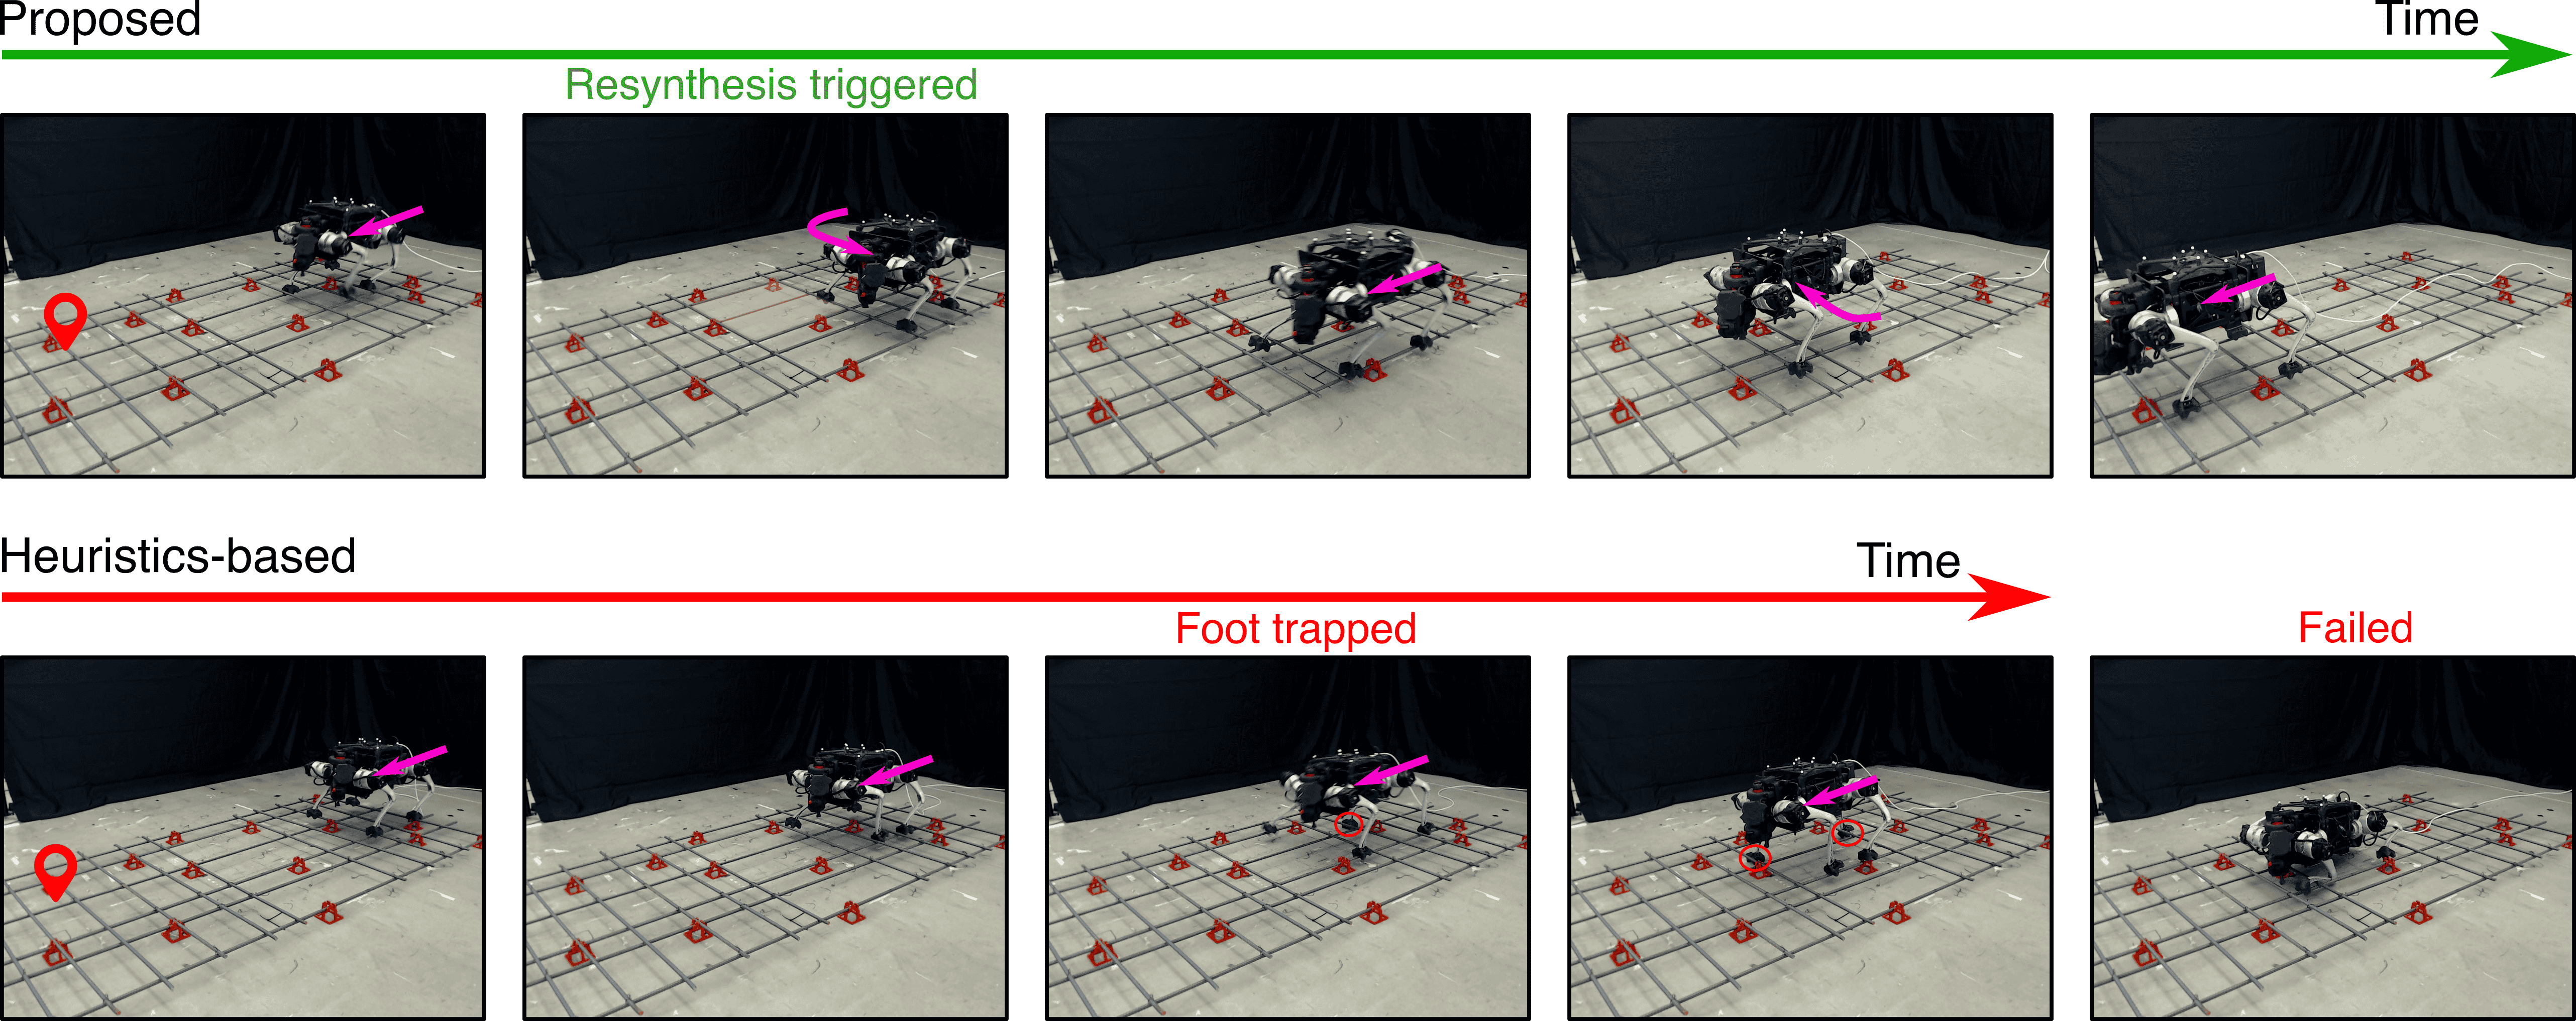
\includegraphics[width=\linewidth]{hardware_rebar_benchmark_compressed.png}
    \caption{Comparison between the proposed method and a heuristics-based planner in an extreme sparse rebar scenario. The proposed method performs resynthesis and succeeds, while the heuristics-based planner fails due to foot trapping.}
    \label{fig:hardware_rebar_benchmark}
\end{figure*}
We create a third rebar scenario, shown in Fig.~\ref{fig:hardware_rebar_benchmark}, by removing two rebars to further increase the maximum spacing to $0.48$ m. This highlights the safety advantage of our planner compared to a heuristics-based footstep planner. The heuristic baseline follows a similar strategy to \citep{fankhauser2018robust, kim2020vision}, adapted for the rebar scenario by selecting the nearest rebar polygon and the closest feasible foothold to a nominal target. The resulting footstep plan and linearly interpolated base trajectory are sent to the same tracking control module. For fairness, all parameters are tuned to achieve successful traversal at a speed of $0.1$ m/s (as shown in the supplemental video).

\revised{We chose this nearest-feasible-foothold heuristic because it isolates the value of feasibility-aware, longer-horizon planning over a single-step heuristic, and because such heuristics remain widely used in deployed perceptive-locomotion stacks due to its computational efficiency. Comparisons against more sophisticated baselines are discussed as future work in Sec.~\ref{sec:discussion}.}

Without re-performing the offline synthesis, our framework directly uses the results from Sec.~\ref{subsec:rebar_terrain}. It classifies the extreme sparse region as an obstacle and performs runtime resynthesis, generating a detour to safely reach the goal. In contrast, we task the heuristics-based planner with the same goal at $0.2$ m/s to match our planner's effective gait speed (i.e., 0.45 m per 2.25 s transition). Without reasoning about the compatibility between terrain geometry and gait feasibility, the heuristic planner suffers from poor EE tracking after a few steps, leading to foot slippage and eventual failure as the robot is entangled by the sparse rebar layout.

\subsection{Computational Time}
We report the hardware computational time in Table~\ref{tab:micp_speed_hardware}. Except for the second scenario in the unstructured terrain, we observe a notable increase in solve time compared to simulation. This is mainly due to two factors: (1) In the first unstructured terrain scenario, the two sets of stepping stones are laterally misaligned from the robot’s viewpoint, requiring non-trivial deviation from the nominal foot location and sideways movement; %\ye{[Does the robot really have a sideway move? It is bit hard to tell in the video.]}\ziyi{[I rephrased it.]} 
(2) In the rebar scenarios, the real-world rebar polygons are not perfectly aligned with the x or y-axis as in simulation, introducing additional numerical complexity for branch-and-bound solvers. Further acceleration of MIP solving through tighter convex relaxations \citep{marcucci2024shortest, lin2024accelerate} remains an important direction for future work.
\begin{table}
\centering
\scriptsize
    \caption{Online Gait-Fixed MICP Solving Time for Hardware}
    \setlength{\tabcolsep}{4pt}
     \begin{tabular}{lccccc}
         \hline
         \textbf{Scenario} &
         \textbf{Polygons} &
         \textbf{Min (s)} &
         \textbf{Mean (s)} &
         \revised{\textbf{Std (s)}} &
         \textbf{Max (s)}\\\hline
         Unstructured - Scene 1 & 6 & 0.81 & 4.04 & \revised{2.50} & 7.86\\
         Unstructured - Scene 2 & 5 & 0.16 & 0.53 & \revised{0.25} & 0.96\\\hline
         Rebar - Scene 1 & 8 & 3.88 & 6.54 & \revised{2.20} & 9.26\\
         Rebar - Scene 2 & 7.5 & 3.60 & 9.13 & \revised{5.50} & 19.23\\
         Rebar - Scene 3 & 6.33 & 2.45 & 7.37 & \revised{4.41} & 14.7\\\hline
    \end{tabular}
    \label{tab:micp_speed_hardware}
\end{table}